\documentclass{ximera}

%\usepackage{todonotes}

\newcommand{\todo}{}

\usepackage{esint} % for \oiint
\ifxake%%https://math.meta.stackexchange.com/questions/9973/how-do-you-render-a-closed-surface-double-integral
\renewcommand{\oiint}{{\large\bigcirc}\kern-1.56em\iint}
\fi


\graphicspath{
  {./}
  {ximeraTutorial/}
  {basicPhilosophy/}
  {functionsOfSeveralVariables/}
  {normalVectors/}
  {lagrangeMultipliers/}
  {vectorFields/}
  {greensTheorem/}
  {shapeOfThingsToCome/}
  {dotProducts/}
  {partialDerivativesAndTheGradientVector/}
  {../productAndQuotientRules/exercises/}
  {../normalVectors/exercisesParametricPlots/}
  {../continuityOfFunctionsOfSeveralVariables/exercises/}
  {../partialDerivativesAndTheGradientVector/exercises/}
  {../directionalDerivativeAndChainRule/exercises/}
  {../commonCoordinates/exercisesCylindricalCoordinates/}
  {../commonCoordinates/exercisesSphericalCoordinates/}
  {../greensTheorem/exercisesCurlAndLineIntegrals/}
  {../greensTheorem/exercisesDivergenceAndLineIntegrals/}
  {../shapeOfThingsToCome/exercisesDivergenceTheorem/}
  {../greensTheorem/}
  {../shapeOfThingsToCome/}
  {../separableDifferentialEquations/exercises/}
  {vectorFields/}
}

\newcommand{\mooculus}{\textsf{\textbf{MOOC}\textnormal{\textsf{ULUS}}}}

\usepackage{tkz-euclide}
\usepackage{tikz}
\usepackage{tikz-cd}
\usetikzlibrary{arrows}
\tikzset{>=stealth,commutative diagrams/.cd,
  arrow style=tikz,diagrams={>=stealth}} %% cool arrow head
\tikzset{shorten <>/.style={ shorten >=#1, shorten <=#1 } } %% allows shorter vectors

\usetikzlibrary{backgrounds} %% for boxes around graphs
\usetikzlibrary{shapes,positioning}  %% Clouds and stars
\usetikzlibrary{matrix} %% for matrix
\usepgfplotslibrary{polar} %% for polar plots
\usepgfplotslibrary{fillbetween} %% to shade area between curves in TikZ
%\usetkzobj{all}
\usepackage[makeroom]{cancel} %% for strike outs
%\usepackage{mathtools} %% for pretty underbrace % Breaks Ximera
%\usepackage{multicol}
\usepackage{pgffor} %% required for integral for loops



%% http://tex.stackexchange.com/questions/66490/drawing-a-tikz-arc-specifying-the-center
%% Draws beach ball
\tikzset{pics/carc/.style args={#1:#2:#3}{code={\draw[pic actions] (#1:#3) arc(#1:#2:#3);}}}



\usepackage{array}
\setlength{\extrarowheight}{+.1cm}
\newdimen\digitwidth
\settowidth\digitwidth{9}
\def\divrule#1#2{
\noalign{\moveright#1\digitwidth
\vbox{\hrule width#2\digitwidth}}}




% \newcommand{\RR}{\mathbb R}
% \newcommand{\R}{\mathbb R}
% \newcommand{\N}{\mathbb N}
% \newcommand{\Z}{\mathbb Z}

\newcommand{\sagemath}{\textsf{SageMath}}


%\renewcommand{\d}{\,d\!}
%\renewcommand{\d}{\mathop{}\!d}
%\newcommand{\dd}[2][]{\frac{\d #1}{\d #2}}
%\newcommand{\pp}[2][]{\frac{\partial #1}{\partial #2}}
% \renewcommand{\l}{\ell}
%\newcommand{\ddx}{\frac{d}{\d x}}

% \newcommand{\zeroOverZero}{\ensuremath{\boldsymbol{\tfrac{0}{0}}}}
%\newcommand{\inftyOverInfty}{\ensuremath{\boldsymbol{\tfrac{\infty}{\infty}}}}
%\newcommand{\zeroOverInfty}{\ensuremath{\boldsymbol{\tfrac{0}{\infty}}}}
%\newcommand{\zeroTimesInfty}{\ensuremath{\small\boldsymbol{0\cdot \infty}}}
%\newcommand{\inftyMinusInfty}{\ensuremath{\small\boldsymbol{\infty - \infty}}}
%\newcommand{\oneToInfty}{\ensuremath{\boldsymbol{1^\infty}}}
%\newcommand{\zeroToZero}{\ensuremath{\boldsymbol{0^0}}}
%\newcommand{\inftyToZero}{\ensuremath{\boldsymbol{\infty^0}}}



% \newcommand{\numOverZero}{\ensuremath{\boldsymbol{\tfrac{\#}{0}}}}
% \newcommand{\dfn}{\textbf}
% \newcommand{\unit}{\,\mathrm}
% \newcommand{\unit}{\mathop{}\!\mathrm}
% \newcommand{\eval}[1]{\bigg[ #1 \bigg]}
% \newcommand{\seq}[1]{\left( #1 \right)}
% \renewcommand{\epsilon}{\varepsilon}
% \renewcommand{\phi}{\varphi}


% \renewcommand{\iff}{\Leftrightarrow}

% \DeclareMathOperator{\arccot}{arccot}
% \DeclareMathOperator{\arcsec}{arcsec}
% \DeclareMathOperator{\arccsc}{arccsc}
% \DeclareMathOperator{\si}{Si}
% \DeclareMathOperator{\scal}{scal}
% \DeclareMathOperator{\sign}{sign}


%% \newcommand{\tightoverset}[2]{% for arrow vec
%%   \mathop{#2}\limits^{\vbox to -.5ex{\kern-0.75ex\hbox{$#1$}\vss}}}
% \newcommand{\arrowvec}[1]{{\overset{\rightharpoonup}{#1}}}
% \renewcommand{\vec}[1]{\arrowvec{\mathbf{#1}}}
% \renewcommand{\vec}[1]{{\overset{\boldsymbol{\rightharpoonup}}{\mathbf{#1}}}}

% \newcommand{\point}[1]{\left(#1\right)} %this allows \vector{ to be changed to \vector{ with a quick find and replace
% \newcommand{\pt}[1]{\mathbf{#1}} %this allows \vec{ to be changed to \vec{ with a quick find and replace
% \newcommand{\Lim}[2]{\lim_{\point{#1} \to \point{#2}}} %Bart, I changed this to point since I want to use it.  It runs through both of the exercise and exerciseE files in limits section, which is why it was in each document to start with.

% \DeclareMathOperator{\proj}{\mathbf{proj}}
% \newcommand{\veci}{{\boldsymbol{\hat{\imath}}}}
% \newcommand{\vecj}{{\boldsymbol{\hat{\jmath}}}}
% \newcommand{\veck}{{\boldsymbol{\hat{k}}}}
% \newcommand{\vecl}{\vec{\boldsymbol{\l}}}
% \newcommand{\uvec}[1]{\mathbf{\hat{#1}}}
% \newcommand{\utan}{\mathbf{\hat{t}}}
% \newcommand{\unormal}{\mathbf{\hat{n}}}
% \newcommand{\ubinormal}{\mathbf{\hat{b}}}

% \newcommand{\dotp}{\bullet}
% \newcommand{\cross}{\boldsymbol\times}
% \newcommand{\grad}{\boldsymbol\nabla}
% \newcommand{\divergence}{\grad\dotp}
% \newcommand{\curl}{\grad\cross}
%\DeclareMathOperator{\divergence}{divergence}
%\DeclareMathOperator{\curl}[1]{\grad\cross #1}
% \newcommand{\lto}{\mathop{\longrightarrow\,}\limits}

% \renewcommand{\bar}{\overline}

\colorlet{textColor}{black}
\colorlet{background}{white}
\colorlet{penColor}{blue!50!black} % Color of a curve in a plot
\colorlet{penColor2}{red!50!black}% Color of a curve in a plot
\colorlet{penColor3}{red!50!blue} % Color of a curve in a plot
\colorlet{penColor4}{green!50!black} % Color of a curve in a plot
\colorlet{penColor5}{orange!80!black} % Color of a curve in a plot
\colorlet{penColor6}{yellow!70!black} % Color of a curve in a plot
\colorlet{fill1}{penColor!20} % Color of fill in a plot
\colorlet{fill2}{penColor2!20} % Color of fill in a plot
\colorlet{fillp}{fill1} % Color of positive area
\colorlet{filln}{penColor2!20} % Color of negative area
\colorlet{fill3}{penColor3!20} % Fill
\colorlet{fill4}{penColor4!20} % Fill
\colorlet{fill5}{penColor5!20} % Fill
\colorlet{gridColor}{gray!50} % Color of grid in a plot

\newcommand{\surfaceColor}{violet}
\newcommand{\surfaceColorTwo}{redyellow}
\newcommand{\sliceColor}{greenyellow}




\pgfmathdeclarefunction{gauss}{2}{% gives gaussian
  \pgfmathparse{1/(#2*sqrt(2*pi))*exp(-((x-#1)^2)/(2*#2^2))}%
}


%%%%%%%%%%%%%
%% Vectors
%%%%%%%%%%%%%

%% Simple horiz vectors
\renewcommand{\vector}[1]{\left\langle #1\right\rangle}


%% %% Complex Horiz Vectors with angle brackets
%% \makeatletter
%% \renewcommand{\vector}[2][ , ]{\left\langle%
%%   \def\nextitem{\def\nextitem{#1}}%
%%   \@for \el:=#2\do{\nextitem\el}\right\rangle%
%% }
%% \makeatother

%% %% Vertical Vectors
%% \def\vector#1{\begin{bmatrix}\vecListA#1,,\end{bmatrix}}
%% \def\vecListA#1,{\if,#1,\else #1\cr \expandafter \vecListA \fi}

%%%%%%%%%%%%%
%% End of vectors
%%%%%%%%%%%%%

%\newcommand{\fullwidth}{}
%\newcommand{\normalwidth}{}



%% makes a snazzy t-chart for evaluating functions
%\newenvironment{tchart}{\rowcolors{2}{}{background!90!textColor}\array}{\endarray}

%%This is to help with formatting on future title pages.
\newenvironment{sectionOutcomes}{}{}



%% Flowchart stuff
%\tikzstyle{startstop} = [rectangle, rounded corners, minimum width=3cm, minimum height=1cm,text centered, draw=black]
%\tikzstyle{question} = [rectangle, minimum width=3cm, minimum height=1cm, text centered, draw=black]
%\tikzstyle{decision} = [trapezium, trapezium left angle=70, trapezium right angle=110, minimum width=3cm, minimum height=1cm, text centered, draw=black]
%\tikzstyle{question} = [rectangle, rounded corners, minimum width=3cm, minimum height=1cm,text centered, draw=black]
%\tikzstyle{process} = [rectangle, minimum width=3cm, minimum height=1cm, text centered, draw=black]
%\tikzstyle{decision} = [trapezium, trapezium left angle=70, trapezium right angle=110, minimum width=3cm, minimum height=1cm, text centered, draw=black]


\title{All Together}

\begin{document}

\begin{abstract}
range
\end{abstract}
\maketitle








Let $L_i(t) = -2t + 1$. \\
Let $L_o(t) = \frac{1}{2}t + 2$.


Let $K(x)$ be a piecewise defined function defined by 


\[
K(x) = 
\begin{cases}
  2|x+6| - 4         &    \,     \text{ on } \,   [-8,-3)    \\
  -6               &    \,     \text{ on } \,    [-3,1)      \\
  -\frac{3}{2}(x-4)(x-6)    &   \,     \text{ on } \,    (4,8]
\end{cases}
\]







\begin{image}
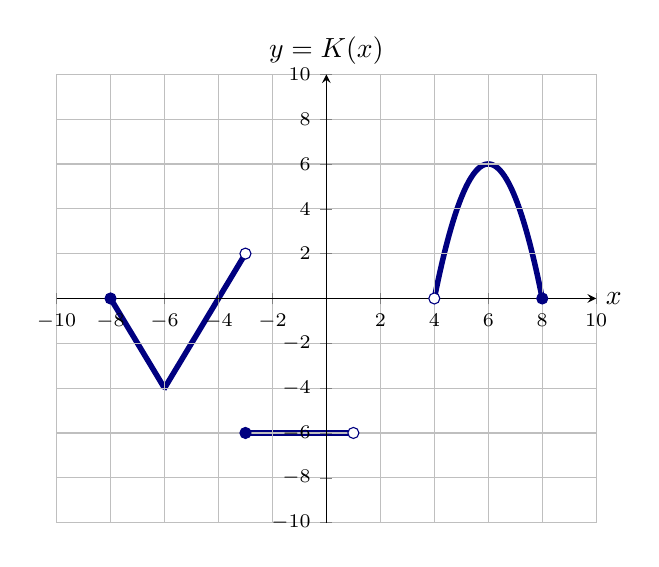
\begin{tikzpicture}
  \begin{axis}[
            domain=-10:10, ymax=10, xmax=10, ymin=-10, xmin=-10,
            axis lines =center, xlabel=$x$, ylabel={$y=K(x)$}, grid = major,
            ytick={-10,-8,-6,-4,-2,2,4,6,8,10},
            xtick={-10,-8,-6,-4,-2,2,4,6,8,10},
            yticklabels={$-10$,$-8$,$-6$,$-4$,$-2$,$2$,$4$,$6$,$8$,$10$}, 
            xticklabels={$-10$,$-8$,$-6$,$-4$,$-2$,$2$,$4$,$6$,$8$,$10$},
            ticklabel style={font=\scriptsize},
            every axis y label/.style={at=(current axis.above origin),anchor=south},
            every axis x label/.style={at=(current axis.right of origin),anchor=west},
            axis on top
          ]
          
          %\addplot [line width=2, penColor2, smooth,samples=100,domain=(-6:2)] {-2*x-3};
            \addplot [line width=2, penColor, smooth,samples=100,domain=(-8:-3)] {2*abs(x+6)-4};
            \addplot[color=penColor,fill=penColor,only marks,mark=*] coordinates{(-8,0)};
          	\addplot[color=penColor,fill=white,only marks,mark=*] coordinates{(-3,2)};

            \addplot [line width=2, penColor, smooth,samples=100,domain=(-3:1)] {-6};
            \addplot[color=penColor,fill=penColor,only marks,mark=*] coordinates{(-3,-6)};
            \addplot[color=penColor,fill=white,only marks,mark=*] coordinates{(1,-6)};

            \addplot [line width=2, penColor, smooth,samples=100,domain=(4:8)] {-1.5*(x-4)*(x-8)};
            \addplot[color=penColor,fill=white,only marks,mark=*] coordinates{(4,0)};
            \addplot[color=penColor,fill=penColor,only marks,mark=*] coordinates{(8,0)};



  \end{axis}
\end{tikzpicture}
\end{image}



This time, we will compose three functions:  $T = L_o \circ K \circ L_i$.


What will be domain (horizontal) effects and range (vertical) effects?  The values $L_i$ will become the inputs to $K$. Therefore, $L_i$ affects the domain of $K$ and moves the graph horizontally.  $L_o$ will take the range values from $K$ and move the graph vertically.



$\blacktriangleright$ Domain - horizontal : $L_i(t) = -2t + 1$


\begin{itemize}
\item The leading coefficient for $L_i$ is negative.  The graph is going to be reflected horizontally. \\
The parabola will be on the left and the ``Vee'' on the right.
\item The leading coefficent is $-2$, which speeds up the input into $K$, which compresses the graph horizontally.
\item Finally, $L_i$ is adding $1$, which is going into $K$, which shifts the graph to the left.

\end{itemize}





$\blacktriangleright$ Range - vertical : $L_o = \frac{1}{2}t + 2$


\begin{itemize}
\item The leading coefficient for $L_o$ is $\frac{1}{2}$.  The graph is going to be compressed vertically. \\
\item Finally, the graph will be shifted up $2$.

\end{itemize}


Graph of $ y = T(m) = (L_o \circ K \circ L_i)(m)$.







\begin{image}
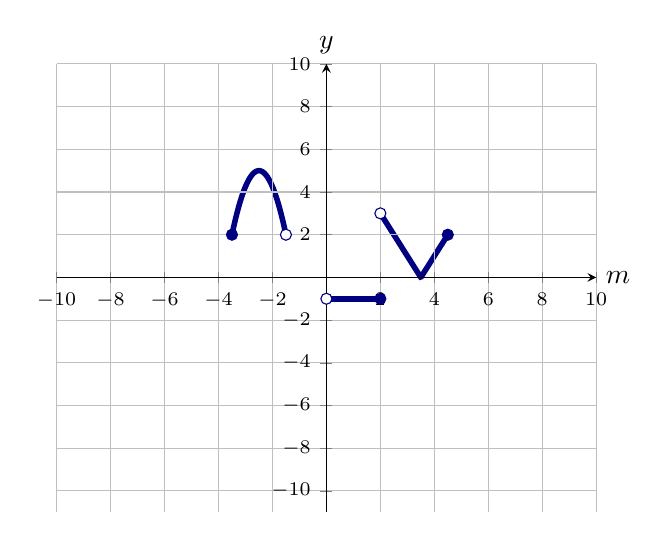
\begin{tikzpicture}
  \begin{axis}[
            domain=-10:10, ymax=10, xmax=10, ymin=-11, xmin=-10,
            axis lines =center, xlabel=$m$, ylabel=$y$, grid = major,
            ytick={-10,-8,-6,-4,-2,2,4,6,8,10},
            xtick={-10,-8,-6,-4,-2,2,4,6,8,10},
            yticklabels={$-10$,$-8$,$-6$,$-4$,$-2$,$2$,$4$,$6$,$8$,$10$}, 
            xticklabels={$-10$,$-8$,$-6$,$-4$,$-2$,$2$,$4$,$6$,$8$,$10$},
            ticklabel style={font=\scriptsize},
            every axis y label/.style={at=(current axis.above origin),anchor=south},
            every axis x label/.style={at=(current axis.right of origin),anchor=west},
            axis on top
          ]
          
          %\addplot [line width=2, penColor2, smooth,samples=100,domain=(-6:2)] {-2*x-3};
            \addplot [line width=2, penColor, smooth,samples=100,domain=(2:4.5)] {abs(-2*x+7)};
            \addplot[color=penColor,fill=white,only marks,mark=*] coordinates{(2,3)};
          	\addplot[color=penColor,fill=penColor,only marks,mark=*] coordinates{(4.5,2)};



            \addplot [line width=2, penColor, smooth,samples=100,domain=(0:2)] {-1};
            \addplot[color=penColor,fill=white,only marks,mark=*] coordinates{(0,-1)};
            \addplot[color=penColor,fill=penColor,only marks,mark=*] coordinates{(2,-1)};



            \addplot [line width=2, penColor, smooth,samples=100,domain=(-3.5:-1.5)] {-0.75*(2*x+3)*(2*x+7)+2};
            \addplot[color=penColor,fill=white,only marks,mark=*] coordinates{(-1.5,2)};
            \addplot[color=penColor,fill=penColor,only marks,mark=*] coordinates{(-3.5,2)};



  \end{axis}
\end{tikzpicture}
\end{image}





\textbf{Note:} All of the endpoints remained the same type.  

\begin{itemize}
\item The short arm of the ``Vee'' is a solid dot on both graphs.
\item The long arm of the ``Vee'' is a hollow dot on both graphs.
\item The end of the horizontal line segment nearest the ``Vee'' is a solid dot on both graphs.
\item The end of the horizontal line segment nearest the parabola is a hollow dot on both graphs.
\item The inside endpoint on the parabola is hollow on both graphs.
\item The outside endpoint on the parabola is solid on both graphs.
\end{itemize}










All horizontal measurements are half what they were, so that when $L_i$ multiplies them by $2$, they get back to their original size for input into $K$.

All height measurements are half what the were to begin with.



We can trace the solid left enpoint of the line segment: $(-3, K(-3)) = (-3, -6)$ on the graph of $K$ through the transformations:





\begin{align*}
\text{Start :} & \text{  } & (-3, K(-3))  \\
\text{Start :} & \text{  } & (-3, -6) \\
\text{Horz Shift Left $1$ :} & \text{  } & (-4,-6)   \\
\text{Horz Reflection :} & \text{  } & (4, -6)   \\
\text{Horz Compress Factor $\tfrac{1}{2}$ :}  & \text{  } & (2, -6)   \\
\text{Vert Compress Factor $\tfrac{1}{2}$:} & \text{  } & (2, -3)   \\
\text{Vert Shift Up $2$ :} & \text{  } & (2, -1)   \\
\text{Composition :} & \text{  } & (2, -1)   
\end{align*}


The solid endpoint of the horizontal line segment will be $(2, -1)$.












\begin{procedure} 



Trace the hollow endpoint of the parabola segment: $(4, 0)$





\begin{align*}
\text{Start :} & \text{  } & (4, K(4))  \\
\text{Start :} & \text{  } & (4, 0) \\
\text{Horz Shift Left $1$ :} & \text{  } & \left( \answer{3}, \answer{0} \right)   \\
\text{Horz Reflection :} & \text{  } & \left( \answer{-3}, \answer{0} \right)   \\
\text{Horz Compress Factor $\tfrac{1}{2}$ :}  & \text{  } & \left( \answer{-\frac{3}{2}}, \answer{0} \right)   \\
\text{Vert Compress Factor $\tfrac{1}{2}$:} & \text{  } & \left( \answer{-\frac{3}{2}}, \answer{0} \right)   \\
\text{Vert Shift Up $2$ :} & \text{  } & \left( \answer{-\frac{3}{2}}, \answer{2} \right)   \\
\text{Composition :} & \text{  } & \left( -\frac{3}{2}, 2 \right)   
\end{align*}


The hollow endpoint of the parabola segment will be $\left( -\frac{3}{2}, 2 \right)$.

\end{procedure}
















\begin{question} 

We know the horizontal line segment remains a horizontal line segment. Therefore the vertical coordinate of the hollow endpoint of the horizontal line segment will become $\answer{-1}$.

\end{question}




  








\begin{procedure} 



Trace the corner of the ``Vee'': $(-6, -4)$





\begin{align*}
\text{Start :} & \text{  } & (-6, K(-6))  \\
\text{Start :} & \text{  } & (-6, -4) \\
\text{Horz Shift Left $1$ :} & \text{  } & \left( \answer{-7}, \answer{-4} \right)   \\
\text{Horz Reflection :} & \text{  } & \left( \answer{7}, \answer{-4} \right)   \\
\text{Horz Compress Factor $\tfrac{1}{2}$ :}  & \text{  } & \left( \answer{\frac{7}{2}}, \answer{-4} \right)   \\
\text{Vert Compress Factor $\tfrac{1}{2}$:} & \text{  } & \left( \answer{\frac{7}{2}}, \answer{-2} \right)   \\
\text{Vert Shift Up $2$ :} & \text{  } & \left( \answer{\frac{7}{2}}, \answer{0} \right)   \\
\text{Composition :} & \text{  } & \left( \frac{7}{2}, 0 \right)   
\end{align*}


The hollow endpoint of the parabola segment will be $\left( \frac{7}{2}, 0 \right)$.

\end{procedure}













\begin{center}
\textbf{\textcolor{green!50!black}{ooooo-=-=-=-ooOoo-=-=-=-ooooo}} \\

more examples can be found by following this link\\ \link[More Examples of Transforming the Outside]{https://ximera.osu.edu/csccmathematics/precalculus1/precalculus1/transformationsOutside/examples/exampleList}

\end{center}


\end{document}
